\normalsize
\section{Receding Boundary Method}


\begin{figure}[h]
  \begin{center}
    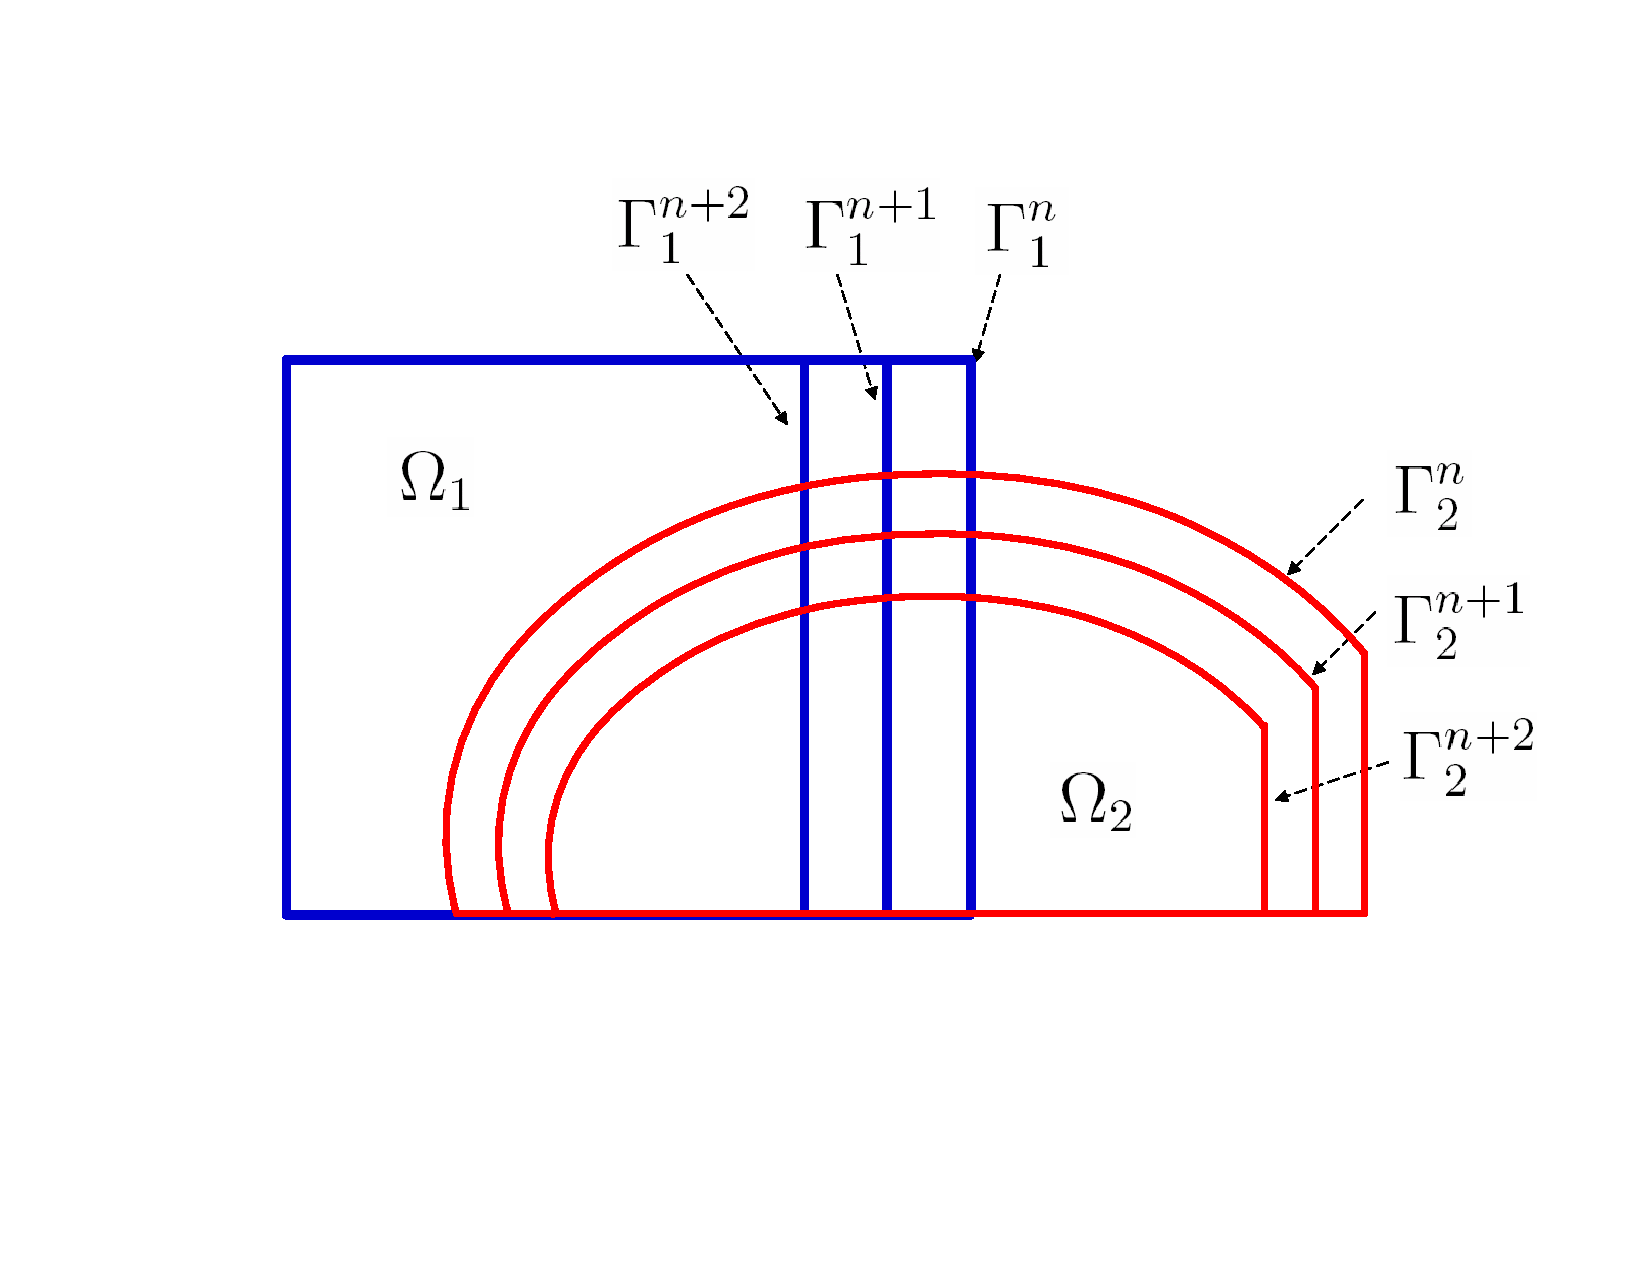
\includegraphics[scale=0.35]{../figures/RecedingBoundaryMethod.pdf}
    \caption{Receding Boundary Method. $\Gamma^n_1$ is the boundary for subdomain $\Omega_1$ at the time step $n$. }
    \label{fig:RecedingBoundaryMethod}
  \end{center}
\end{figure}

The receding boundary method (RBM) is an approximate domain decomposition technique for incompressible computational fluid dynamics. While dividing the computational domain into smaller subdomains, RBM utilizes an overlapping, receding grid strategy to enable the independent solution of each subdomain.

The two main features of the receding boundary method are as follows:
(1) On the subdomain boundaries, the receding boundary method assumes a open boundary condition for the pressure. In the gravity current application the derivative of pressure is assumed to be zero on the subdomain boundary. There are both advantages and disadvantages to this assumption. The advantage is that it allows each subdomain to independently solve the pressure Poisson equation. The disadvantage is that on the subdomain boundaries, there is no non-hydrostatic correction for the velocities normal to the boundaries. This will result in inaccurate corrections for the velocities perpendicular to the boundaries and further affect corrections in all parts of each subdomain. Besides, the errors of the velocities on the boundaries will be carried inside through the advection and diffusion.

\begin{figure}[p]
  \begin{center}
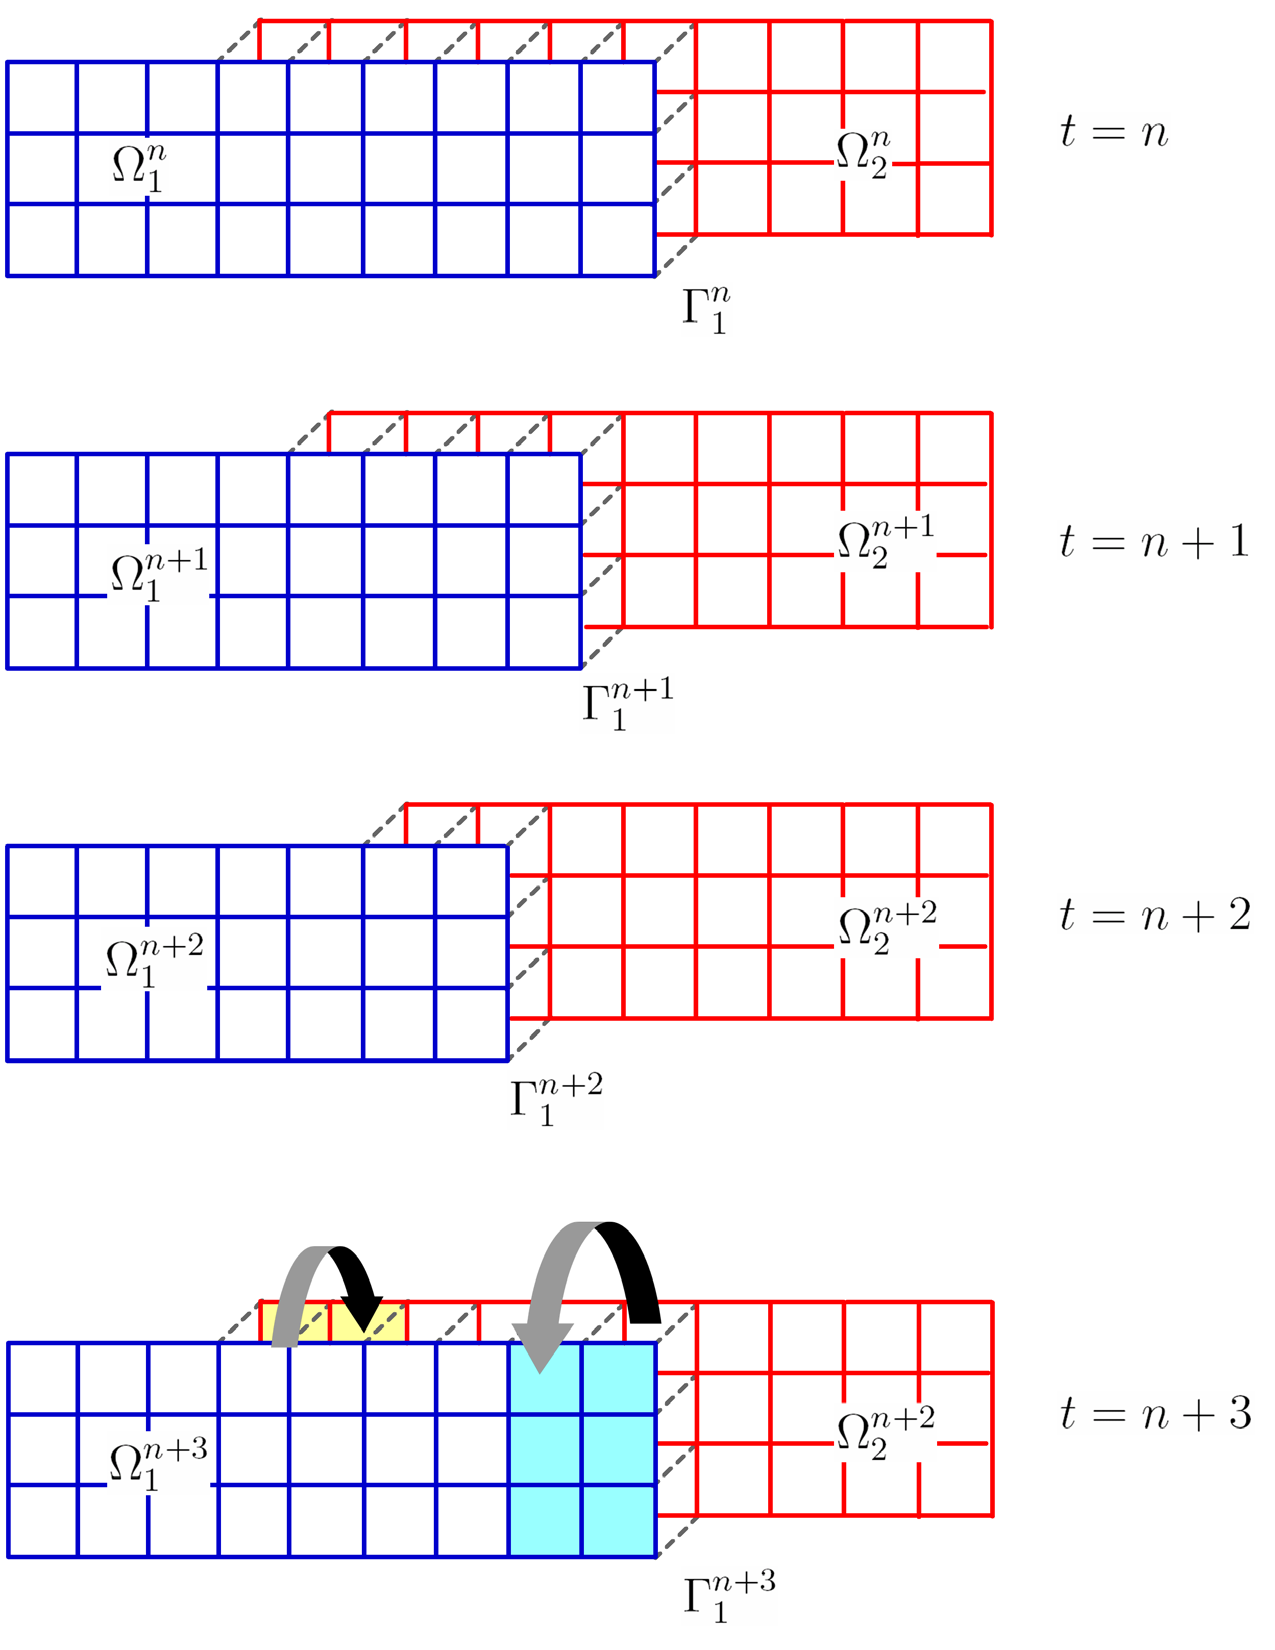
\includegraphics[scale=0.52]{../figures/RecedingBoundaryMethod-Grid.pdf}
    \caption{Subdomain boundaries continue to move inward for a few time steps and then reset to the original location.}
    \label{fig:RecedingBoundaryMethod-Grid}
  \end{center}
\end{figure}

(2) To mitigate the errors caused by the assumed open boundary condition for the pressure, the receding boundary method makes subdomain boundaries in the overlapping regions non-stationary. They continue to move inward for a few time steps and then reset to the original location. When the boundary is receding, the open boundary condition is applied at least one grid point inward for every time step. This prevents the repeated use of the open boundary condition on the same location, thus deceases the accumulation of the errors on the subdomain boundaries. In addition, the inward transport of errors is also decreased because the information outside the receding boundaries is discarded. However, continuing to recede the subdomain boundaries will shrink the subdomain size and eventually the overlapping regions of the subdomains will vanish. Therefore the subdomain boundaries are reset to the original location every few time steps. The missing information on the reset area of one subdomain is obtained from the other subdomains, and this is when the communication between subdomains occurs. %RBM is presented in this chapter for a gravity current example which belongs to the incompressible flow regime. However, the application of this domain decomposition technique is not limited to incompressible cases and may be experimented with compressible flow in the future.


\subsection{Open Boundary Conditions}
The first feature of RBM is the assumption of open boundary conditions on the overlapping subdomain boundaries divided from the whole domain. The purpose of open boundary conditions is to minimize the effect of the fictitious boundaries defined by the computational modeling. In Figure \ref{fig:RBM-step1}, it shows a staggered grid example of two overlapping subdomains. The open boundary condition is applied at the cell-centered pressure variable and the velocity variable at the subdomain boundary. With this assumption, the dynamic pressure Poisson equation in each subdomain is solved independently without communications. After the pressure Poisson equation is solved, the predicted velocity field is corrected by the dynamic pressure in each subdomain. Some reviews and numerical tests of different open boundary conditions can be found in the references, \cite{Sani1994, Jensen1998, Stevens1990, Camerlengo1980, Palma1998}.

\subsubsection*{\normalsize{Derivative Boundary Condition} }
The derivative boundary condition is a commonly used technique. On the artificial boundary, the first derivative of some quantity $\Phi$ is assumed to be zero:
\begin{equation}
\partial \Phi /\partial x = 0
\end{equation}
Numerically the value $\Phi$ on the boundary is not computed. Rather, it's extrapolated from inner grid points.
For supercritical outflow, this technique does not cause erroneous reflection because the information only travels downstream. However, this non-reflecting behavior is not guaranteed for subcritical outflow. Nordstrom \cite{Nordstrom1995} shows that if large gradients tangential to the artificial boundary are present, then accurate solutions can be obtained in the subcritical outflow case.

\subsubsection*{\normalsize{Radiation Boundary Condition}}
The radiation boundary condition \cite{Sommerfeld1949} allows the
interior wave to pass freely through the artificial boundary with
a known phase speed.
Numerically the value on the boundary is updated by the information transmitted
from inner domain with the phase speed $c$:
\begin{equation}
\frac{\partial \Phi}{\partial t}-c\frac{\partial \Phi}{\partial x}
= 0
\end{equation}
This radiation boundary condition performs well if the advection term is dominated by the phase speed $c$ and it is known exactly.
A modified version \cite{Orlanski1976} suggests the effective phase speed be evaluated at each time step. A two dimensional version \cite{Engquist1977} generalizes to wave angles other than normal incidence. Higdon \cite{Higdon86} uses the product of the operator in the Sommerfeld condition to further reduce wave reflection.
\subsubsection*{\normalsize{Characteristics-Based Boundary Condition}}
Characteristics-based techniques \cite{Henderson1966} use inward and outward Riemann variables to solve for the artificial boundary. The flow velocity is included in the advection term. Besides, the flow condition outside the artificial boundary is specified and thus also affect the boundary values.
For example, in one dimensional open channel flow the velocity and water depth at the artificial boundary can be computed as:
\begin{equation}
u=(R^+_L + R^-_R)/2
\end{equation}
\begin{equation}
h=(R^+_L - R^-_R)^2/16g
\end{equation}
\subsubsection*{\normalsize{Absorbing/Damping Boundary Condition}}
The damping boundary condition \cite{Kosloff1986} treats the
near-boundary region with a high viscosity to dissipate waves. Therefore the interior is less affected by the reflecting wave. Similar concepts  \cite{Petropoulos1998, Shin1995} are applied to attenuate reflected waves for simulations of Maxwell's equations and seismic waves.
\subsubsection*{\normalsize{Relaxation Boundary Condition}}
The relaxation type boundary condition forces the solution $\Phi$ at the near boundary region to a specified value $\Phi_{specified}$ with a relaxation parameter $w$ varies from $1$ to $0$. This parameter normally decreases from the boundary to the inner domain. A review article discussing this boundary condition in weather prediction models is written by Davies\cite{Davies1983}. Martinsen and Engedahl \cite{Martinsen1987} also use this type of boundary condition in a barotropic ocean model.
\begin{equation}
\Phi_{adjusted} = (1-w)\Phi + w\Phi_{specified}
\end{equation}


\begin{figure}[h]
  \begin{center}
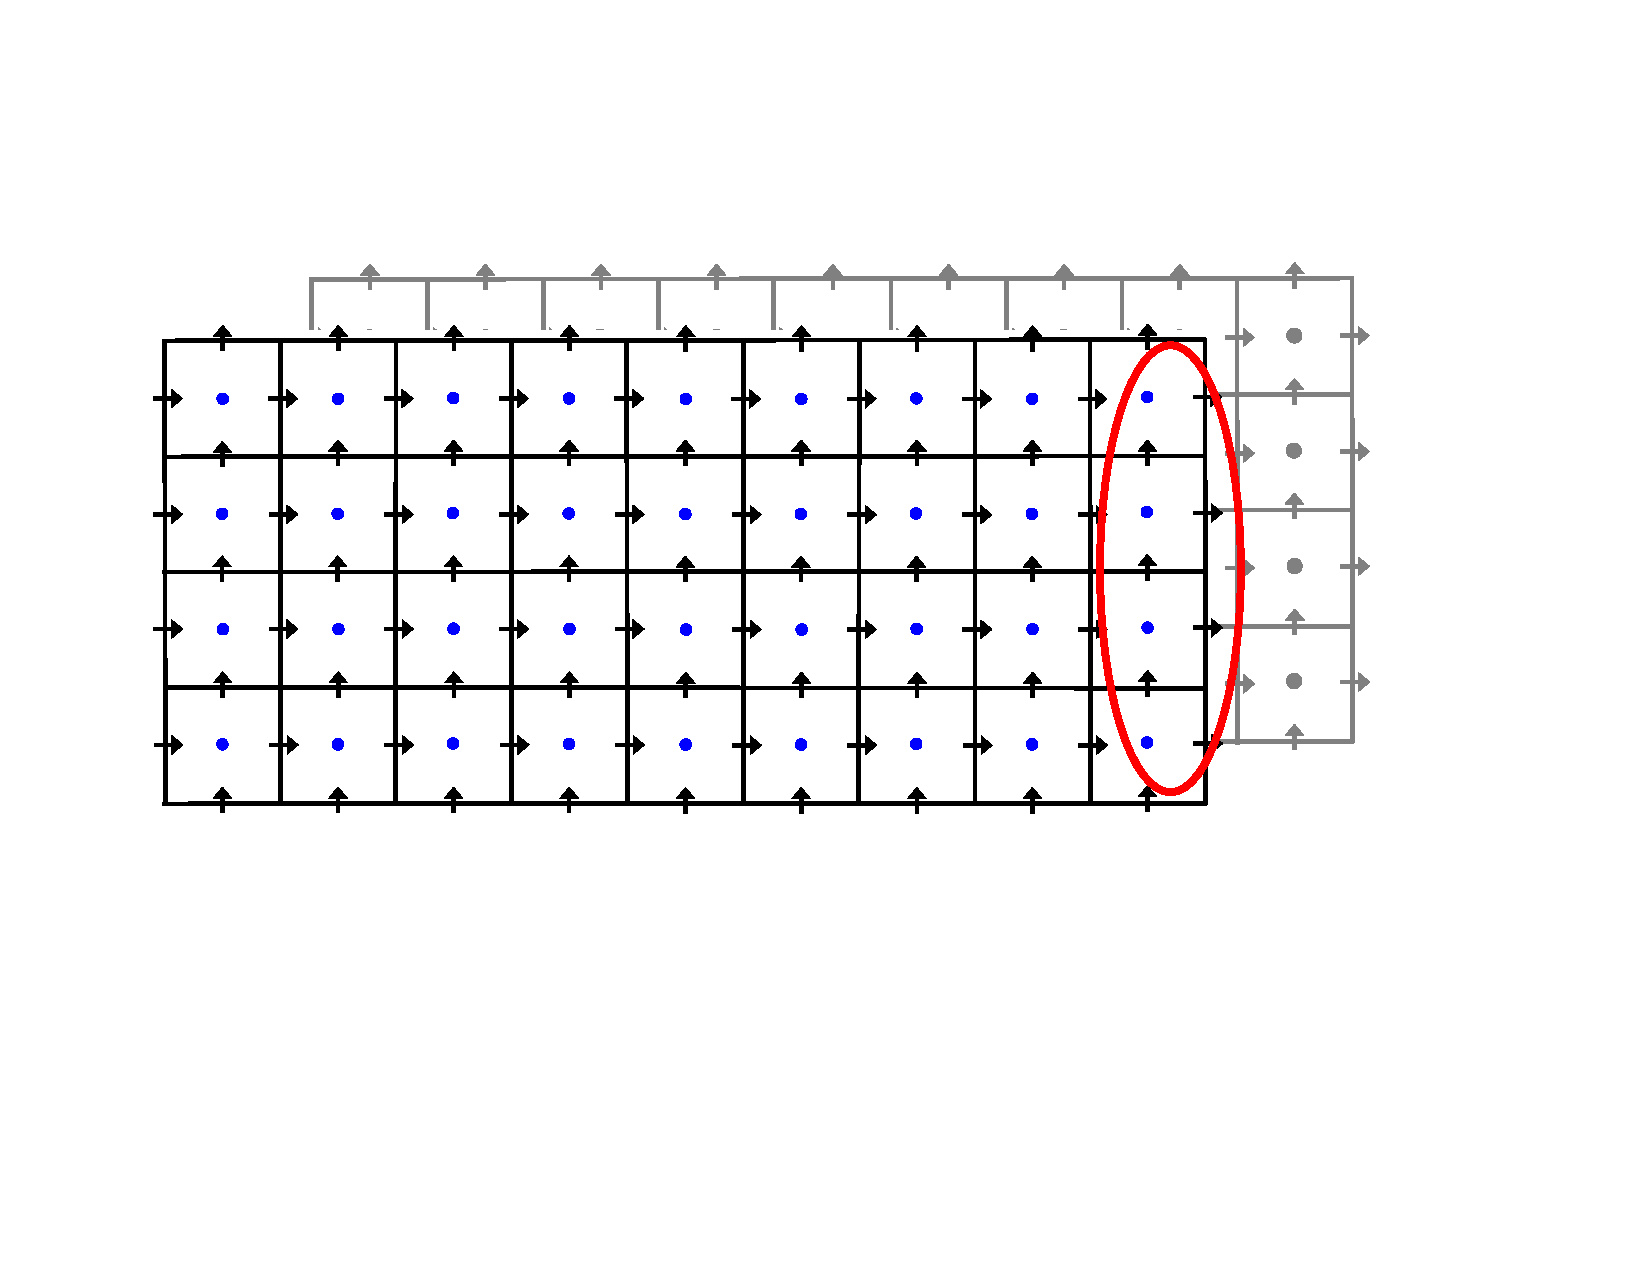
\includegraphics[scale=0.4]{../figures/RBM-step1.pdf}
   \caption{This figure shows the overlapping parts of two subdomains. The open boundary condition is applied on the subdomain boundaries, which enables the independent solution for each subdomains.}
    \label{fig:RBM-step1}
  \end{center}
\end{figure}

\subsection{Receding Subdomain Boundary}

The second feature of this method is the receding, or inward-moving of subdomain boundaries. This is intended to exclude the information close to the assumed open boundary condition. This receding method can reduce the error of incomplete velocity field correction caused by the open boundary assumptions.

In Fig \ref{fig:RBM-step2}, the subdomain boundaries recede two grids from Fig \ref{fig:RBM-step1} after the dynamic pressure Poisson equation is solved and the velocity field is corrected. This receding process can be repeated many times. However, the subdomains must remain overlapping leastwise. To illustrate the concept of receding boundary, the whole domain is decomposed into two subdomains as shown in Fig. \ref{fig:RecedingBoundaryMethod-Grid}, Fig. \ref{fig:RBM-step1} and Fig. \ref{fig:RBM-step2}. To show the location of the subdomain boundaries in the sense of grid index, we can define the following terms:

\begin{itemize}
\item $X_{reset}$ is the reset location (in the sense of grid index of $x$-axis direction) of the subdomain boundaries; this reset location is the same as the initial location which gives the maximum overlapping area.
\item $X_{mid}$ is the midpoint (also in the sense of grid index of $x$-axis direction) between the two overlapping subdomain boundaries; the two overlapping subdomains will shrink to un-overlapping subdomains when their boundaries recede beyond this location.
\item The buffer $B$ is half the number of grids between the two overlapping subdomain boundaries; in other words, $B$ gives the number of grids between $X_{mid}$ and one of the subdomain boundary.
\item $G$ is the receding rate, or how fast the subdomain boundaries recede in the unit of grids per receding step.
\item Finally the number of computational steps of each resetting-receding cycle is defined as subiteration $S$; to keep the two subdomains overlapping, subiteration $S$ should be limited by the allowable receding range, e.g., $S<B/G$.
\end{itemize}

Therefore at the $n-th$ computational step counting from the boundary reset, the boundary location $X_{R}$ of the front subdomain (as shown in Fig. \ref{fig:RBM-step2}) and the boundary location $X_{L}$ of the other subdomain can be written as:
\ba
X_{R} = X_{mid} - B + (n-1)*G \\
X_{L} = X_{mid} + B - (n-1)*G
\ea
At the end of each resetting-receding cycle, the boundary locations are
\ba
X_{R\_end} = X_{mid} - B + (S-1)*G \\
X_{L\_end} = X_{mid} + B - (S-1)*G
\ea
and the subdomain boundaries reset after every computational steps of $S$,
\ba
X_{R\_reset} = X_{mid} - B \\
X_{L\_reset} = X_{mid} + B
\ea


\begin{comment}
   NX1B_ = InterX - buffer + ratio*Receding
   NX1E_ = NX

Interpolation
i_up = InterX+Buffer-Subiteration*Receding  ! +1 !(10+4-2*1=12)
i_low = InterX-Buffer+subiteration*Receding ! -1 !(10-4+2*1=8)

\end{comment}

\begin{figure}[htbp]
  \begin{center}
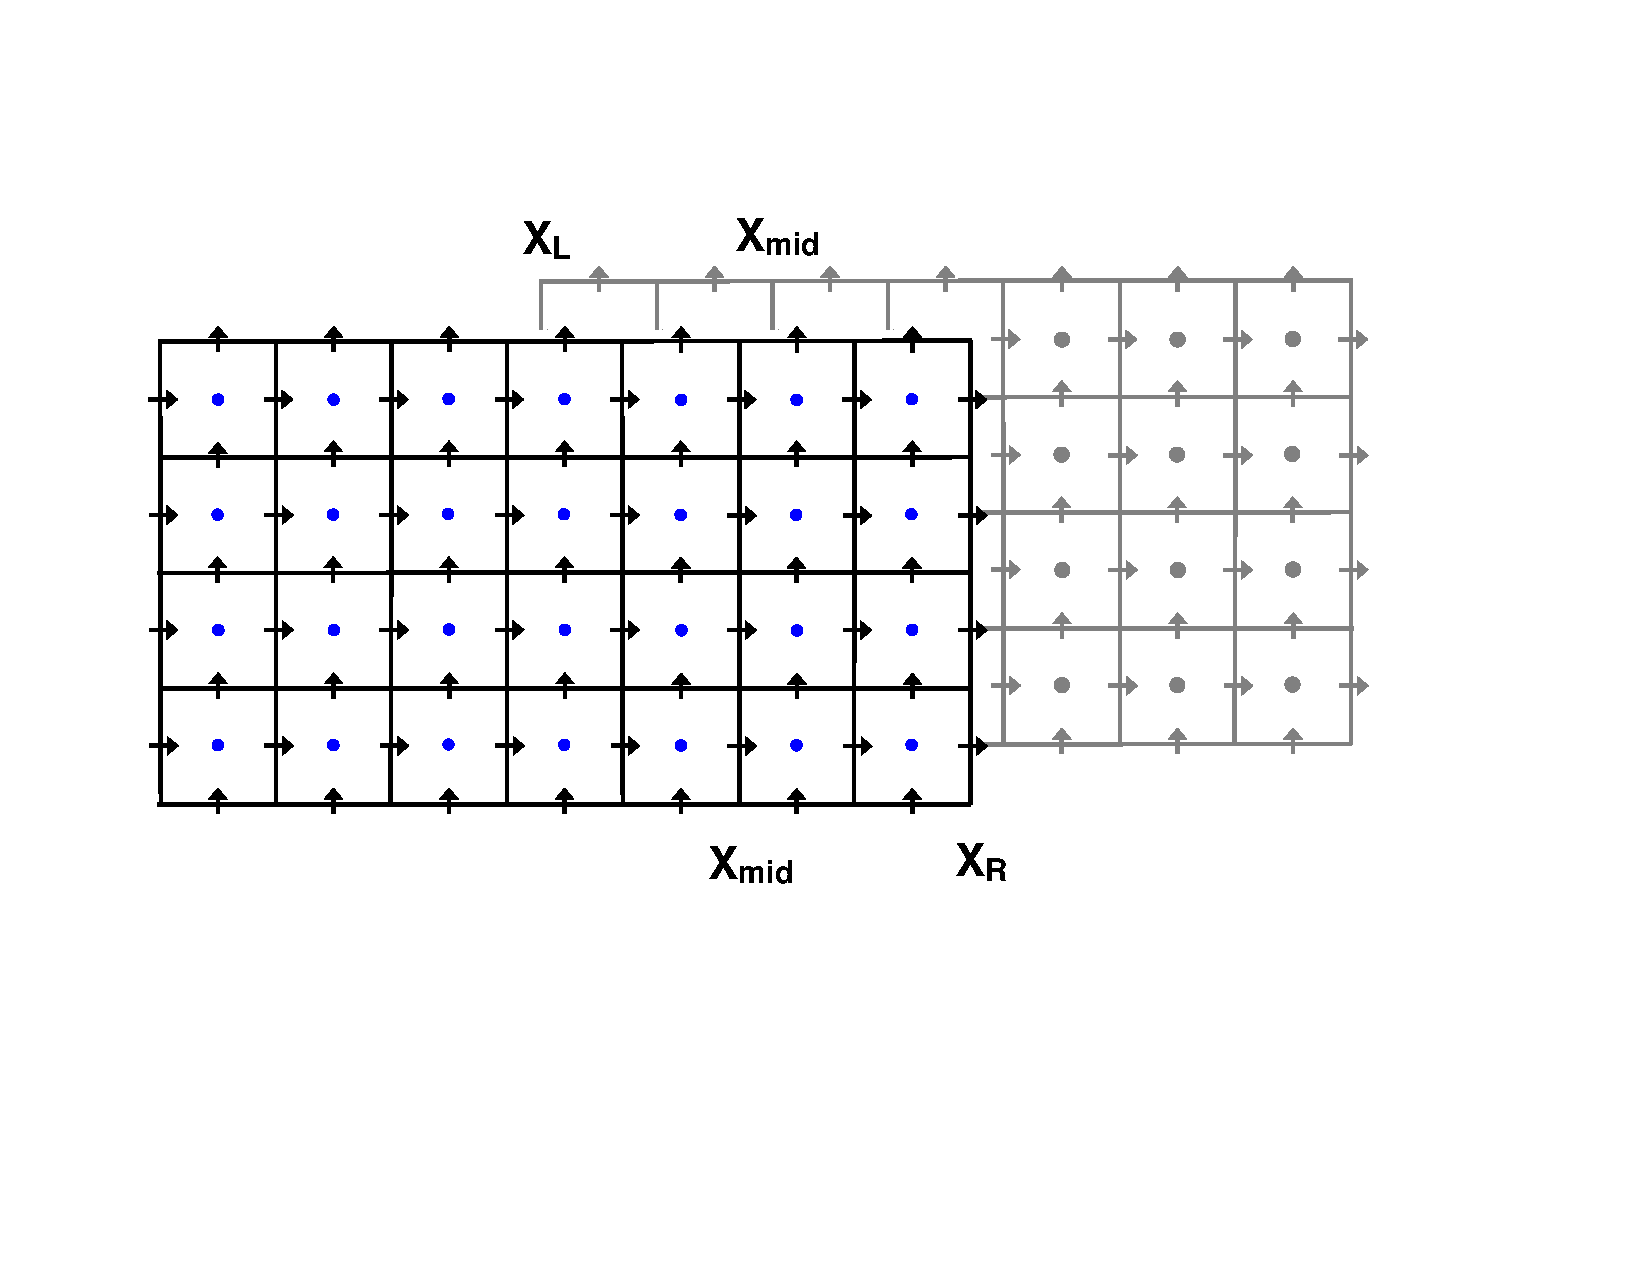
\includegraphics[scale=0.4]{../figures/RBM-step2.pdf}
   \caption{This figure shows the midpoint $X_{mid}$ of the two overlapping subdomain boundaries, $X_R$ and $X_L$. The boundaries recede two grids from Fig. \ref{fig:RBM-step1}. This receding of subdomain boundaries reduces the error resulted from the assumption of open boundary conditions.}
    \label{fig:RBM-step2}
  \end{center}
\end{figure}


\subsection{Stabilization for Overlapping Subdomains}
\label{chapter:RBM-Smoothing}

The third feature of RBM is the stabilization of the overlapping grids after reset of subdomain boundaries. The information of the reset grids can be simply copied from the other overlapping subdomain, but different subdomain will probably have different solutions on the overlapping grids and such treatment might produce discontinuities. To prevent the solutions of subdomains from diverging, the information can be averaged from those overlapping subdomains by some interpolation method. Common interpolation methods include linear interpolation, polynomial interpolation, spline interpolation, rational interpolation, and trigonometric interpolation. However, in our case we are dealing with the interpolation of matrices with essentially non-linear behavior inherited from the Navier-Stokes equation, and the discussion of optimized interpolation method is beyond this work's scope. The linear interpolation is used for simplicity in the gravity current examples to smooth the transition from the overlapping part to the inner subdomains.

\begin{figure}[htbp]
  \begin{center}
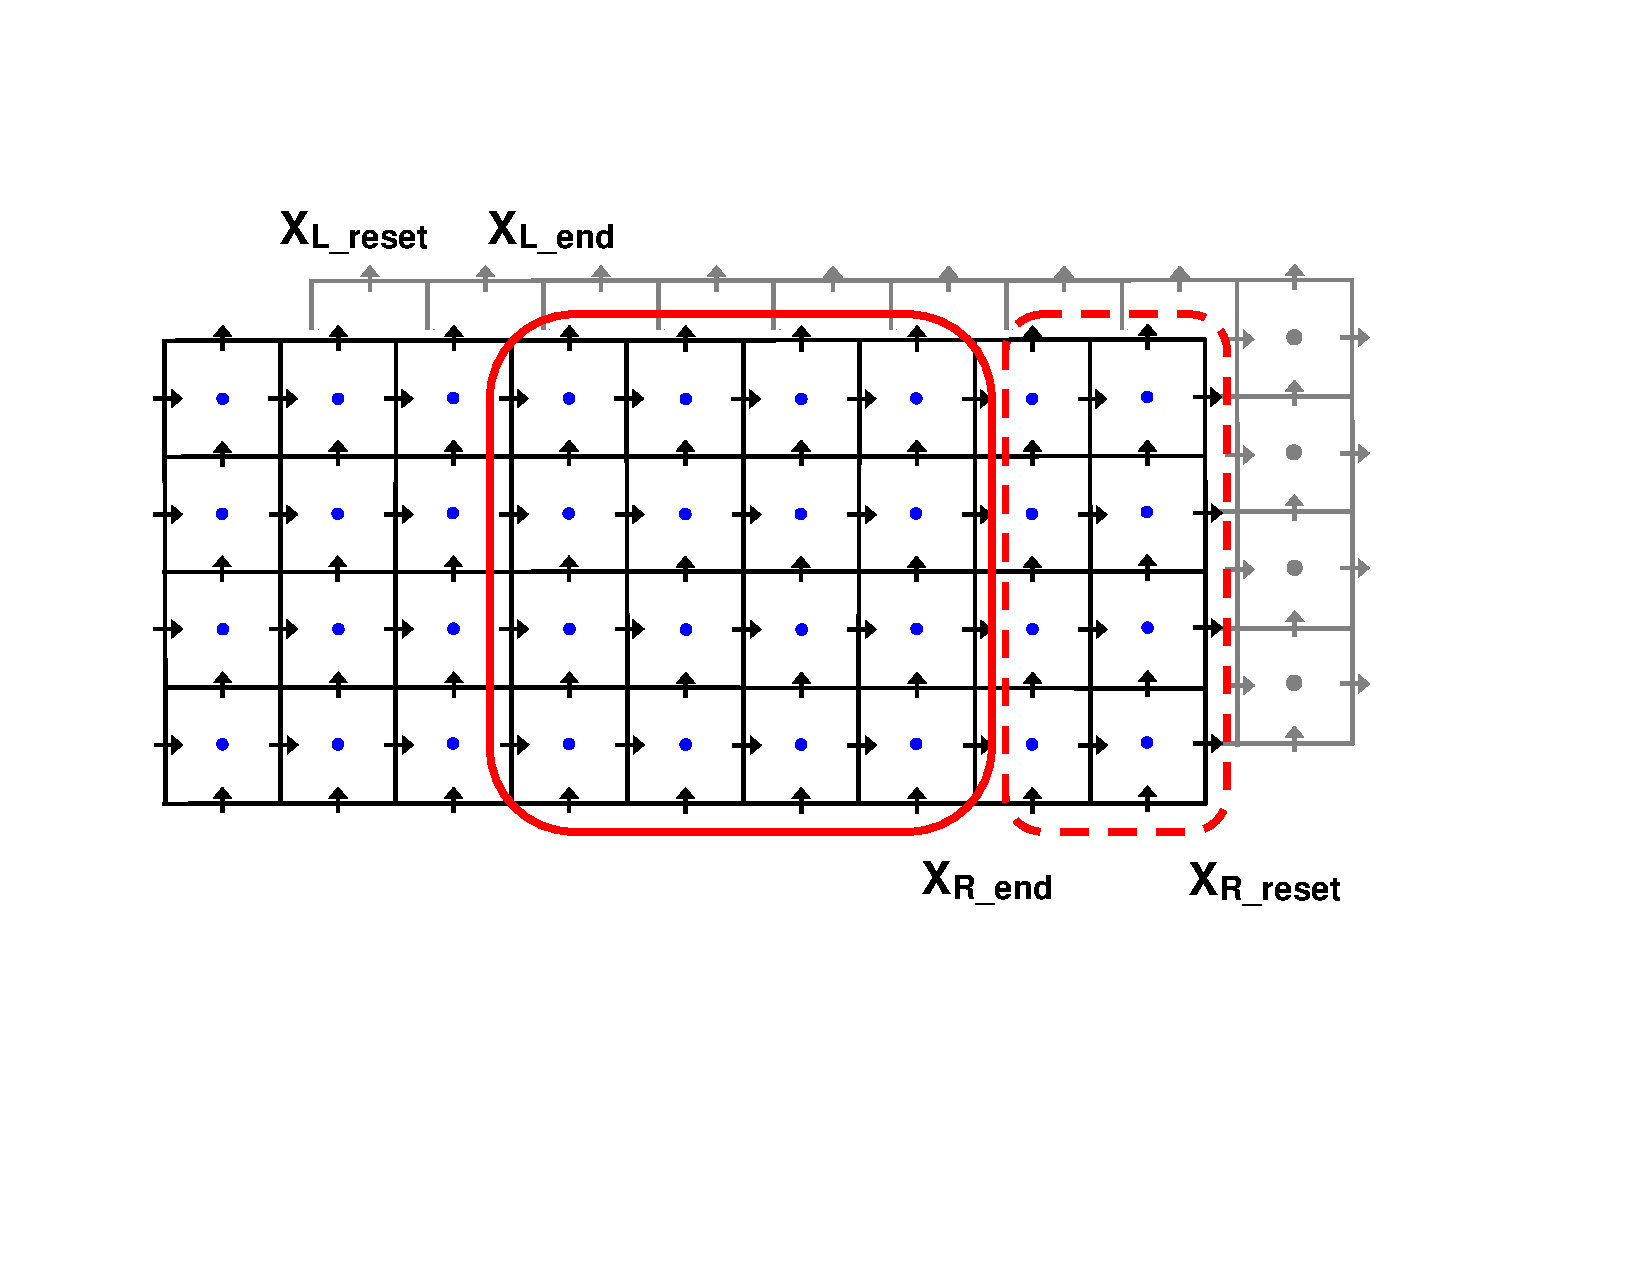
\includegraphics[scale=0.4]{../figures/RBM-step3.pdf}
   \caption{The left-hand-side subdomain boundary recedes from $X_{R\_reset}$ to $X_{R\_end}$ and then back to $X_{R\_reset}$. After reset, in the area surrounded by dotted line the information is copied from the other subdomain. In the area surrounded by solid line, the information is linearly averaged by the two subdomains. The weighting factor is design to reduce the effect of open boundary assumptions. }
    \label{fig:RBM-step3}
  \end{center}
\end{figure}

In the example Figure \ref{fig:RBM-step3}, The left-hand-side subdomain boundary recedes from $X_{R\_reset}$ to $X_{R\_end}$ and then back to $X_{R\_reset}$. The variables $\Phi_{reset}$ on the overlapping grids between $X_{R\_end}$ and $X_{L\_end}$ (as shown circled by the solid line) are averaged by the solutions $\Phi_{R}$ and $\Phi_{L}$ from two overlapping subdomains:
\begin{equation}
\Phi_{reset} = w_R \Phi_{R} + w_L \Phi_{L}
\end{equation}
The weighting factors $w_R$ and $w_L$ are designed to decrease the influence of the open boundary assumptions:
\be
w_R = \f{X - X_{L\_reset} }{X_{R\_reset}-X_{L\_reset}}
\ee
\be
w_L = \f{X_{R\_reset} - X }{X_{R\_reset}-X_{L\_reset}}
\ee

Between $X_{R\_end}$ and $X_{R\_reset}$ the information is copied from the left-hand-side subdomain, and between $X_{L\_end}$ and $X_{L\_reset}$ the information is copied from the right-hand-side subdomain:
\be
\Phi_{reset}=\left\{
\baa{ccc}
\Phi_{L}      & if & X > X_{R\_end} \\
\Phi_{R}      & if & X < X_{L\_end}
\eaa
\right.
\ee














%The drawback is that discontinuity will occur if the value of the overlapping part is simply copied from one subdomain. They can be weighted by the distance to the subdomain boundary, by the upwind velocity, or both.

%The linear interpolation method is used to smooth the overlapping area.


%!(linear)
%!NXBdum = NX_begin_D2-1; NXEdum = INT(0.5*(NX_end_D2 + NX_begin_D1))
%!WRITE(*,*) 'domain 2 NXBdum, NXEdum', NXBdum,NXEdum  ! 0 12
%!NXBdum=0;NXEdum=12
%! (1) i>= i_up = InterX+Buffer-Subiteration*Receding(10+4-2*1=12)
%!    uu_1=uu_2 = uut_1

%! (2) i_up>i>i_low
%!    uu_1=uu_2 = uut_1* weight1 + uut_2 * weight2
%!    weight1= ABS(i-i_low)/ABS(i_low-i_up)
%!    weight2= ABS(i-i_up)/ABS(i_low-i_up)

%!    i= InterX
%!    uu_1=uu_2=(uut_1+uut_2)/2

%! (3) i<= i_low = %InterX-Buffer+subiteration*Receding(10-4+2*1=8)
%!    uu_1=uu_2 = uut_2

%\section{numerical test}

%without free surface. The can be applied to the Baroclinic mode or interior simulation.
